\chapter{App}
\label{ch:app}

Da die App Kamerafunktionen verwendet, wird auf dem Smartphone ein \acrshort{api}-Level von 21 vorausgesetz. Dies entspricht Android 5.0, welches 2014 erschienen ist.

\section{Aufbau}
\begin{figure}[htpb]
    \centering
    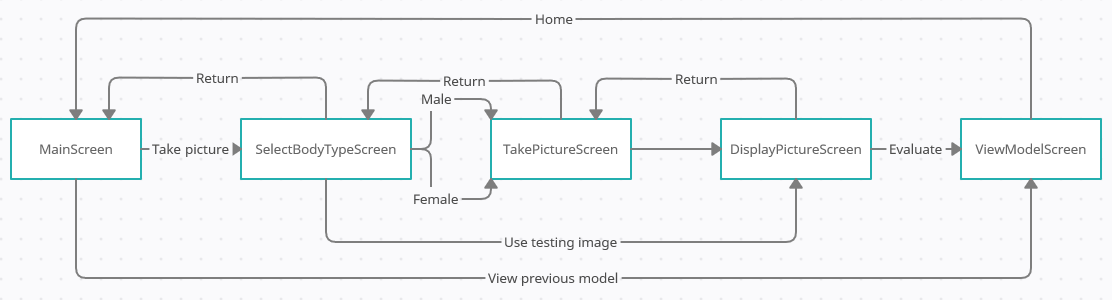
\includegraphics[width=1\textwidth]{appflowchart}
    \caption{Programmablauf der App}
    \label{img:appflowchart}
\end{figure}

In \ref{img:appflowchart} ist der Programmablauf der App dargestellt. Die einzelnen Screens und deren Funktionen werden in den folgenden Abschnitten erläutert. \newline
Da das Design kein Hauptmerkmal der Anwendung ist, wurde eine simple Benutzeroberfläche erstellt. Diese beruht auf einem Dark-Design und setzt Akzente in Blau.

\pagebreak
\section{MainScreen}
\label{sec:mainscreen}
\begin{figure}[htpb]
    \centering
    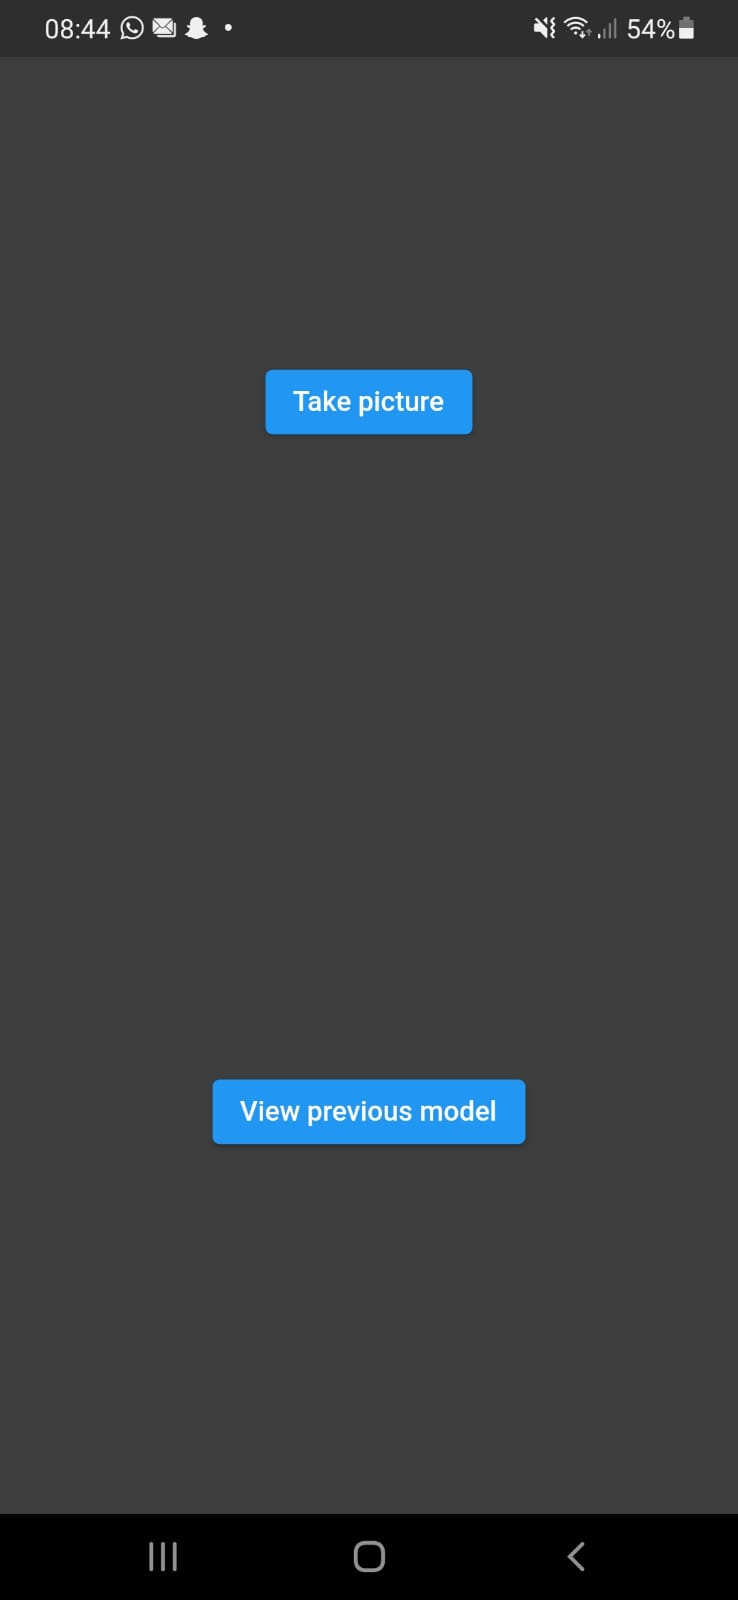
\includegraphics[width=0.3\textwidth]{mainscreen}
    \caption{Der Mainscreen der App}
    \label{img:mainscreen}
\end{figure}

\begin{figure}[htpb]
    \centering
    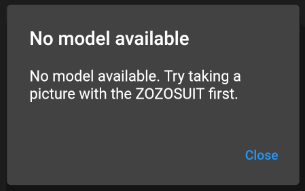
\includegraphics[width=0.7\textwidth]{nomodel}
    \caption{Error-Message}
    \label{img:nomodel}
\end{figure}

Der Startbildschirm der Anwendung (\ref{img:mainscreen}) verfügt über zwei Buttons: \glqq{}Take picture\grqq{} und \glqq{}View previous model\grqq{}. \newline
Mit \glqq{}View previous model\grqq{} wird der ViewModelScreen (\ref{img:viewmodel}) aufgerufen und das zuletzt generierte 3D-Modell angezeigt. Befindet sich auf dem Gerät 
kein zuvor generiertes Modell, so wird ein Popup mit einer Error-Message angezeigt (\ref{img:nomodel}). Diese weißt darauf hin, dass kein Modell vorhanden ist und dieses somit zuerst 
durch Aufnehmen und Auswerten eines Fotos generiert werden muss.

Sobald der Startbildschirm generiert wird, werden die auf dem Smartphone verfügbaren Kameras gescannt und in einer Liste gespeichert. Aus dieser Liste wird die Rückkamera 
ausgelsesen und gespeichert. Die Kamera wird später in \ref{sec:takepicture} benötigt. Das Auslesen und Auswerten der Gerätekameras kann etwas Zeit in Anspruch nehmen, weshalb dies 
bereits im Mainscreen passiert und nicht erst beim Aufrufen von TakePictureScreen.

Wird der Button \glqq{}Take picture\grqq{} gedrückt, so wird der SelectBodyTypeScreen generiert und diesem die zuvor gespeicherte Kamera übergeben.

\clearpage
\section{SelectBodyTypeScreen}
\begin{figure}[htpb]
    \centering
    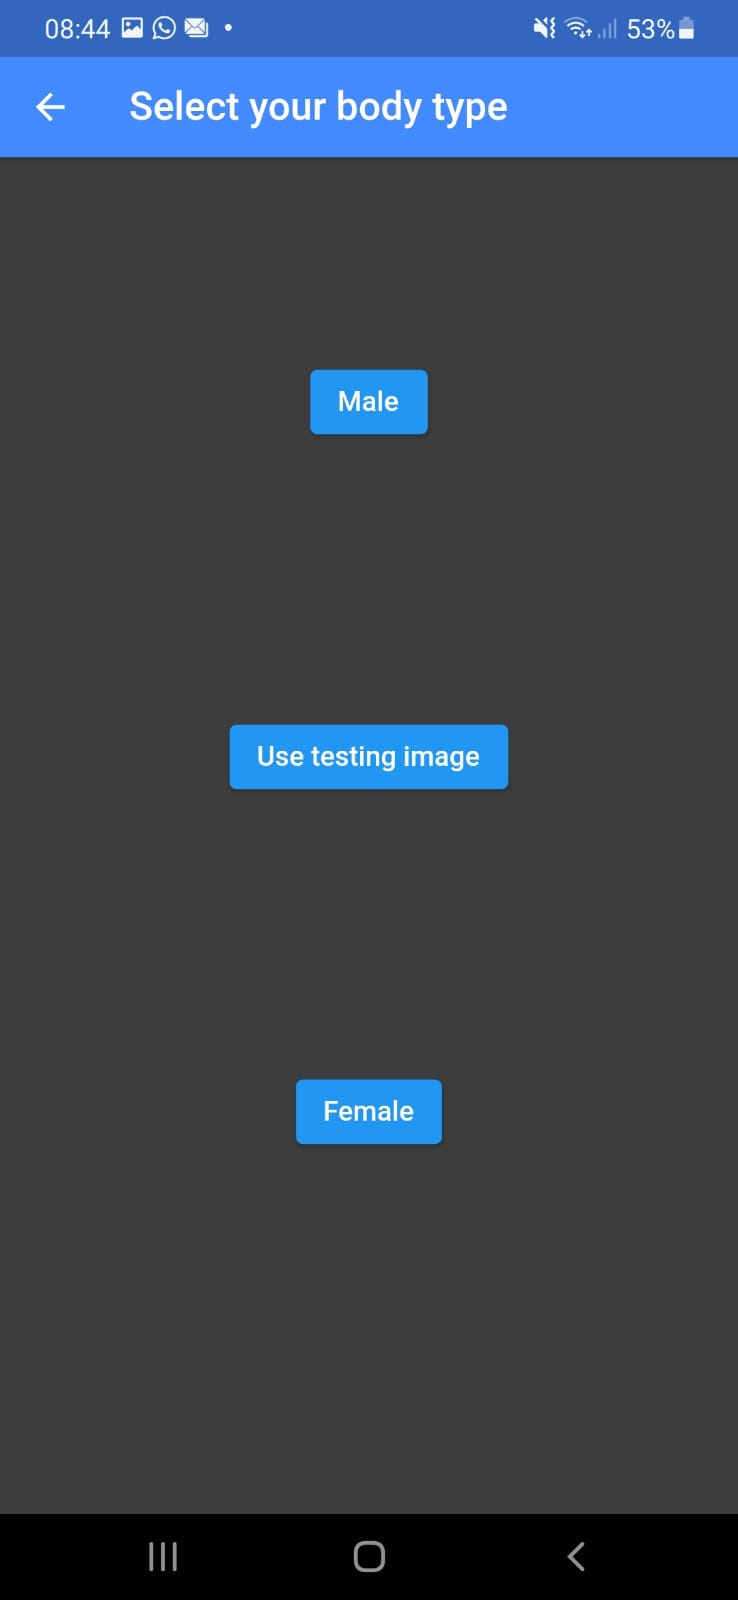
\includegraphics[width=0.3\textwidth]{selectbodytype}
    \caption{Auswahl des Körpertyps}
    \label{img:selectbodytype}
\end{figure}

Auf dem SelectBodyTypeScreen sind drei Buttons vorhanden: \glqq{}Male\grqq{}, \glqq{}Use testing image\grqq{} und \glqq{}Female\grqq{}. Zusätzlich ist eine Statusleiste vorhanden, 
welche zurück zum vorherigen Screen leitet.

Der Button \glqq{}Use testing image\grqq{} leitet den Nutzer direkt zum DisplayPictureScreen (\ref{sec:displaypicture}). Dort wird ein Beispielbild eines Entwicklers in der ZOZOSUIT 
angezeigt, welches anschließend ausgewertet werden kann. \newline
Diese Funktion ist sinnvoll, wenn man die Anwendung testen will und keinen eigenen ZOZOSUIT besitzt oder wenn man den Prozess des An- und Ausziehens des ZOZOSUIT umgehen will.

Die Buttons \glqq{}Male\grqq{} und \glqq{}Female\grqq{} leiten den Nutzer zum TakePictureScreen weiter. Hierbei wird die Variable \textit{gender} übergeben, welche bei der Generierung 
des 3D-Modells benötigt wird. Das drücken eines Buttons setzt dabei die Variable auf das dem Button entsprechende Geschlecht.

\clearpage
\section{TakePictureScreen}
\label{sec:takepicture}
\begin{figure}[htpb]
    \centering
    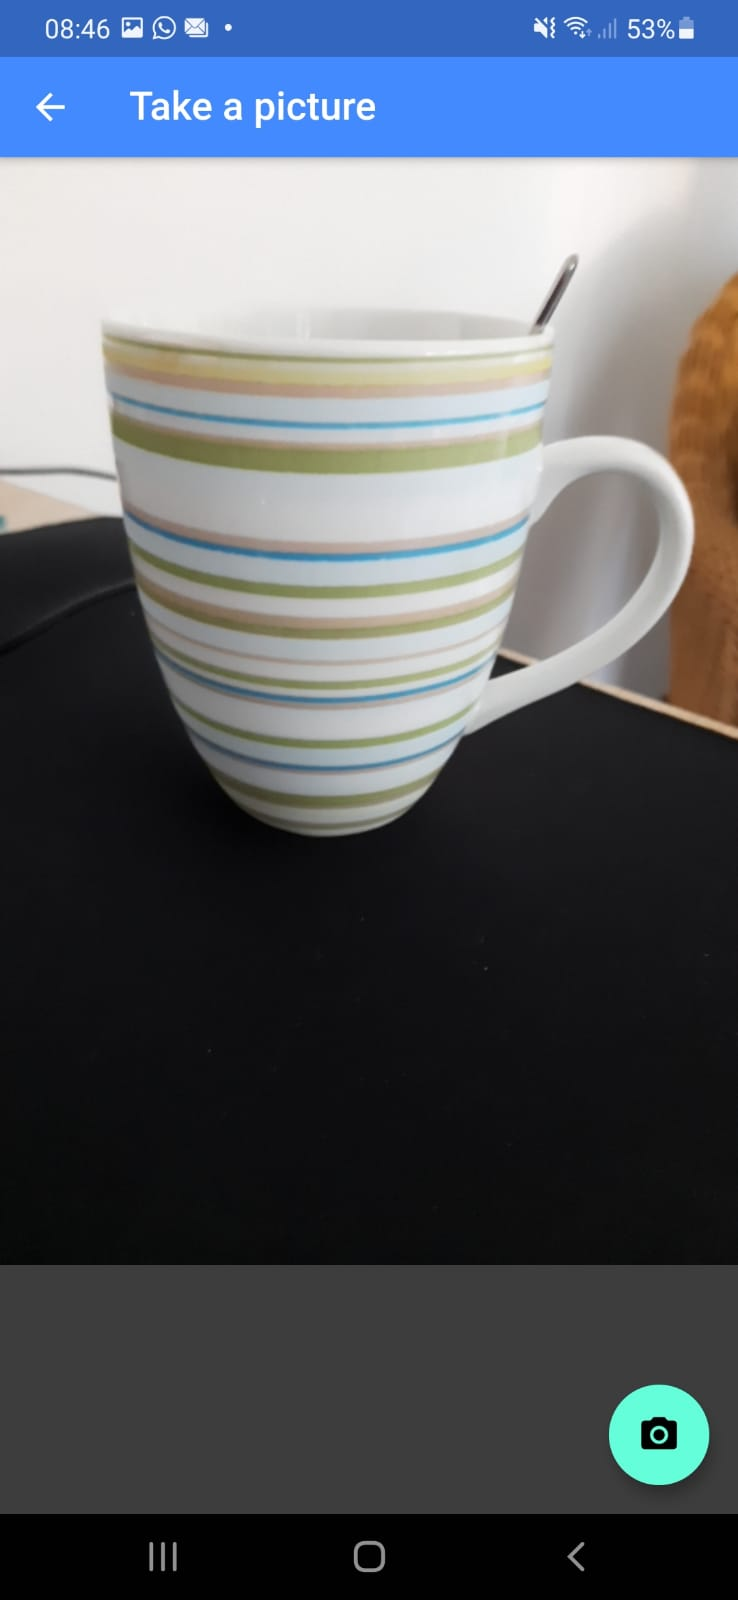
\includegraphics[width=0.3\textwidth]{takepicture}
    \caption{Aufnehmen eines Bildes}
    \label{img:takepicture}
\end{figure}

Der TakePictureScreen verfügt über einen Button mit einem Kamerasymbol und eine Statusleiste, welche den Nutzer zum vorherigen Screen leitet.

In der Mitte des Bildschirms wird der aktuelle Kamerafeed der Rückkamera angezeigt, welche bereits in \ref{sec:mainscreen} bereitgestellt wurde. Wird der Kamerabutton gedrückt, 
so wird ein Bild aufgenommen und temporär gespeichert. Der Pfad zum aktuellen Bild und das vom SelectBodyTypeScreen erhaltene Geschlecht werden an den DisplayPictureScreen weitergeleitet, 
welcher nun generiert wird.

\clearpage
\section{DisplayPictureScreen}
\label{sec:displaypicture}
\begin{figure}[htpb]
    \centering
    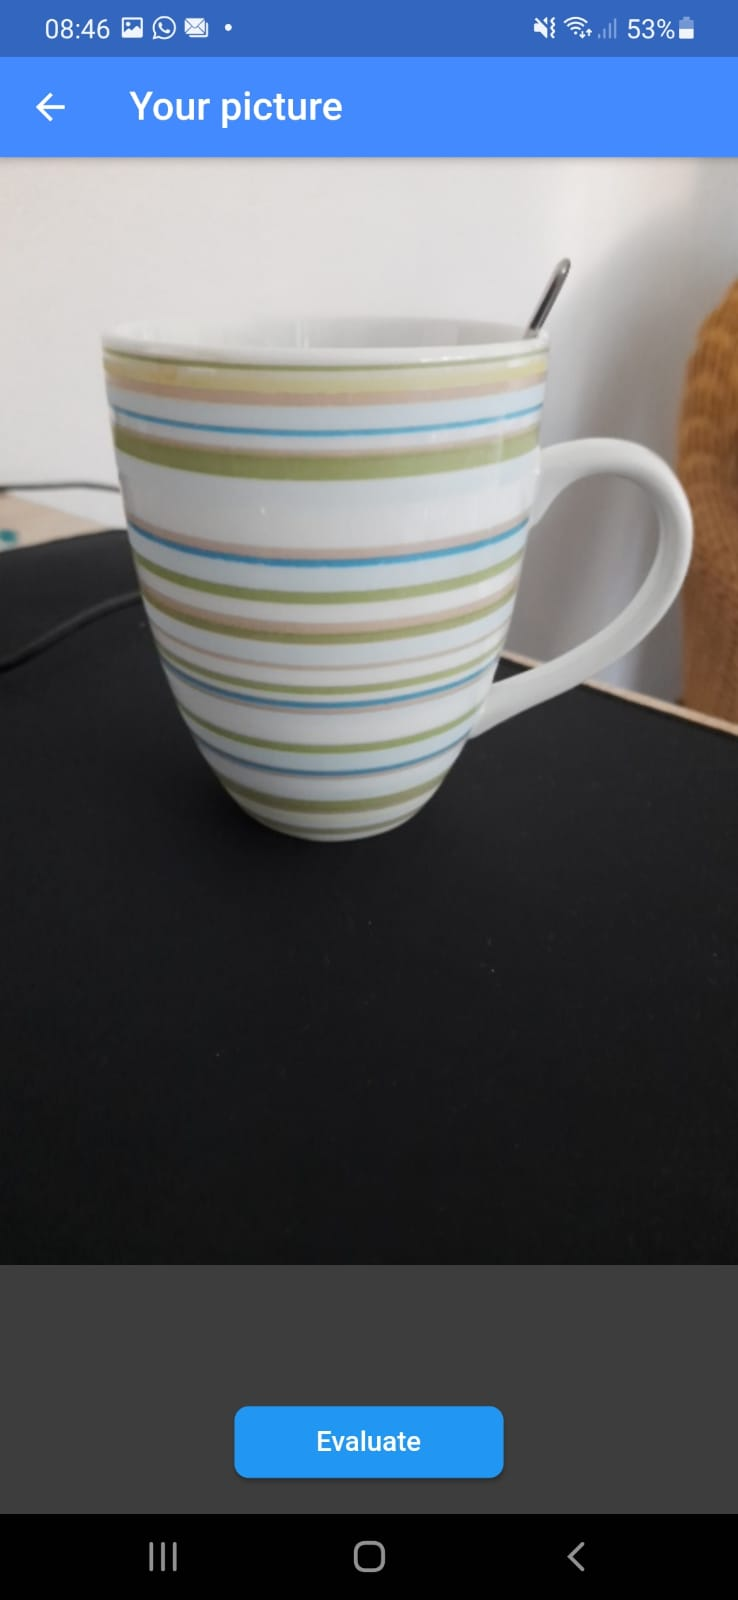
\includegraphics[width=0.3\textwidth]{displaypicture}
    \caption{Anzeigen des aufgenommenen Bildes}
    \label{img:displaypicture}
\end{figure}

Der DisplayPictureScreen zeigt das zuvor aufgenommene Bild an und besitzt den Button \glqq{}Evaluate\grqq{} und eine Statusleiste, welche den Nutzer zum vorherigen Screen leitet. \newline
Wurde im SelectBodyTypeScreen der Button \glqq{}Use test image\grqq{} gedrückt, so wird eine Variante dieses Screens angezeigt. Der einzige Unterschied liegt dabei darin, dass nicht 
das zuvor aufgenommene Bild, sondern ein aus den, in der App enthaltenen, Assets geladenes Bild, angezeigt wird.

Wird der Button gedrückt, so zeigt dieser eine Ladeanimation an, bis alle durch den Button aufgerufenen Funktionen abgeschlossen sind.

Zuerst wird das aktuelle Bild zu einem Base64-String (\cite{misc:base64}) konvertiert. Der somit generierte String wird nun mit dem erhaltenen Geschlecht per POST-Request an den Server 
gesendet. Der Server wertet die Daten aus und generiert daraus ein 3D-Modell als .glb-Datei. Diese Datei wird zu Base64 kodiert und an die App zurückgesendet. \newline
Der Base64-String wird nun dekodiert und in dem appspezifischen Speicher gespeichert. Hierbei muss darauf geachtet werden, dass die Speicherorte auf Android und iOS Geräten 
verschieden sind. Deshalb wird das Betriebssystem des Smartphones bestimmt und daraus lässt sich der Pfad zum Speicherort für appspezifische Dateien generieren. Die dekodierte Datei 
wird nun an dem erhaltenen Pfad gespeichert. \newline
Der Pfad zum gespeicherten 3D-Modell (die .glb Datei) wird gespeichert und an den ViewModelScreen weitergegeben, welcher nun generiert wird.

\clearpage
\section{ViewModelScreen}
\begin{figure}[htpb]
    \centering
    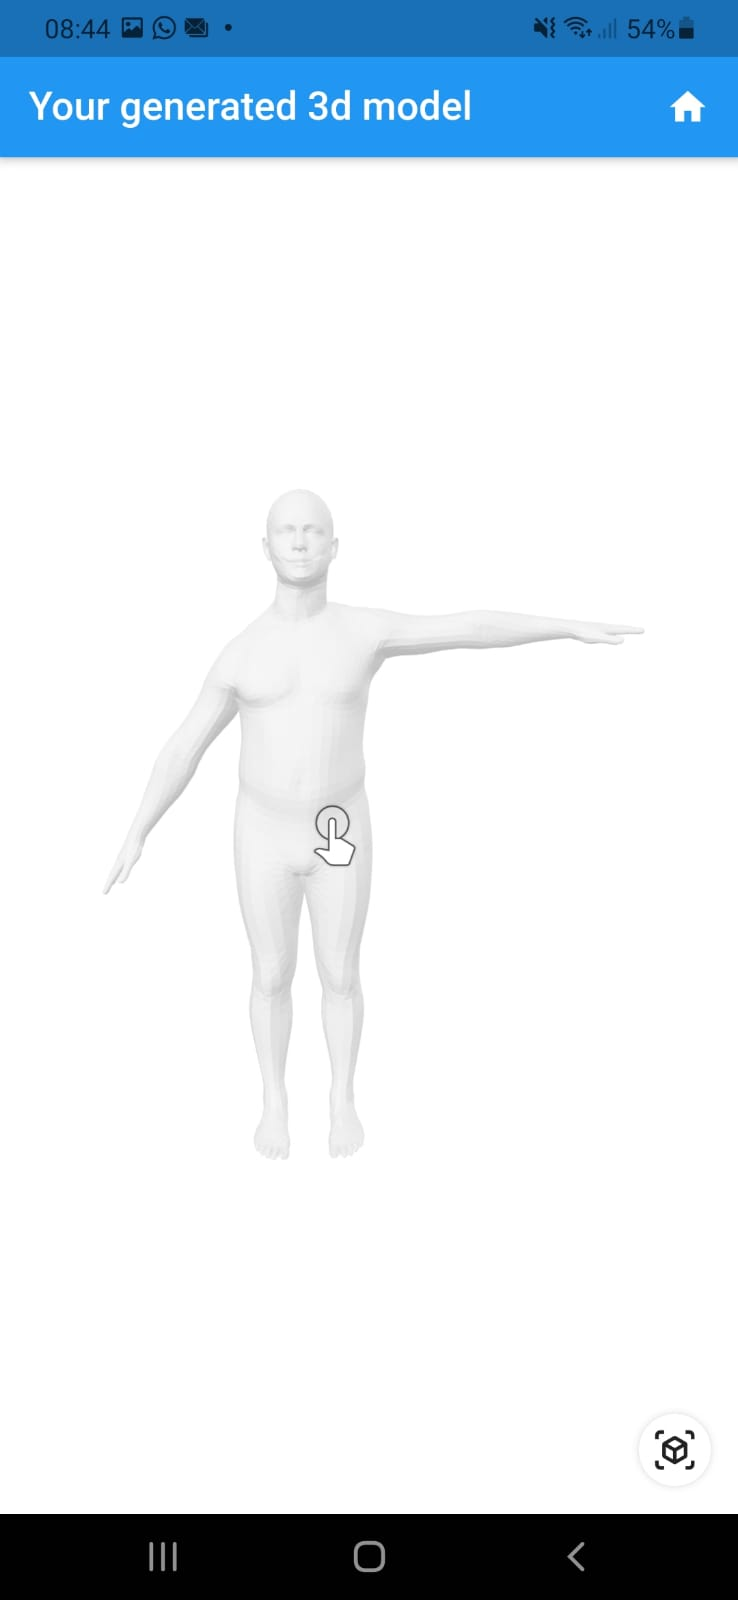
\includegraphics[width=0.3\textwidth]{viewmodel}
    \caption{Anzeigen des 3D-Modells}
    \label{img:viewmodel}
\end{figure}

Der ViewModelScreen erhält einen Pfad zu einer .glb-Datei. Diese Datei wird gerendert und als drehbares 3D-Modell gerendert. Zusätzlich ist eine Statusleiste mit einem Home-Button 
vorhanden, welcher den Nutzer zurück zum MainScreen bringt. 

Um das 3D-Modell zu rendern verwendet die App das Plugin \textit{Model Viewer} (\cite{misc:modelviewer}). \textit{Model Viewer} erstellt eine WebView und startet somit einen Server 
innerhalb der App. Das 3D-Modell wird in einem Browser mithilfe von WebGL gerendert und in der App dargestellt.

Der Button rechts unten lädt das Modell im von Google erstellten model-viewer, auf welchem dieses Plugin basiert.

\pagebreak
\section{Probleme}

